\synctex=1
\documentclass[a4paper,10.1pt,svgnames]{book}
\usepackage{cite}
\usepackage[utf8x]{inputenc}
\usepackage{mathtools}
\usepackage{thesis}
\usepackage{calc}
\usepackage{float}
\usepackage{acronym}
\usepackage{siunitx}
\usepackage{eurosym}
\usepackage{indentfirst}
\usepackage{bookmark}
\usepackage{blindtext}
\usepackage[titletoc]{appendix}
\usepackage[acronym]{glossaries}

% \makeglossaries
\renewcommand{\UrlFont}{\ttfamily\footnotesize}

\setcounter{secnumdepth}{5}
\setcounter{tocdepth}{5}


% \usepackage[backend=biber,
% style=apa]{biblatex}

% \renewcommand{\familydefault}{\sfdefault}

% \renewcommand{\contentsname}{Contenidos}
% \renewcommand{\listfigurename}{Lista de Figuras}
% \renewcommand{\chaptername}{Capítulo}
% \renewcommand{\figurename}{Figura}
% \renewcommand{\bibname}{Referencias}
% \renewcommand{\appendixname}{Anexo}
% \renewcommand{\tablename}{Tabla}

% \setlength{\marginparwidth}{2cm}
% \setlength{\voffset}{-0.25in}
\setlength{\parskip}{0.1in}

% \usepackage{draftwatermark}
% \SetWatermarkScale{4}
\usepackage{subfig}
\usepackage{listings}
\usepackage{courier}
\usepackage{enumitem}
% \usepackage{indentfirst}

\lstset{
    basicstyle=\footnotesize\ttfamily,
    numbers=none,              
    numberstyle=\tiny,         
    % stepnumber=2,            
    numbersep=5pt,              
    tabsize=2,                
    extendedchars=true,       
    breaklines=true,            
    % keywordstyle=\color{red},
    frame=single,         
    % keywordstyle=[1]\textbf,   
    % keywordstyle=[2]\textbf,    
    % keywordstyle=[3]\textbf,    
    % keywordstyle=[4]\textbf,   
    % stringstyle=\color{white}\ttfamily, 
    showspaces=false,          
    showtabs=false,             
    belowcaptionskip=12pt,
    xleftmargin=2em, 
    xrightmargin=4pt,
    % backgroundcolor=\color{lightgray},
    showstringspaces=false,      
    aboveskip=5pt,
    belowskip=10pt
 }
 
 \lstloadlanguages{% Check Dokumentation for further languages ...
    % [Visual]Basic
    % Pascal
    % C
    C++,
    XML,
    % HP
    Java,
    bash
 }
 
% \usepackage{xcolor}
\usepackage[usenames,dvipsnames,table]{xcolor}

\colorlet{punct}{red!60!black}
\definecolor{background}{HTML}{FFFFFF}
\definecolor{delim}{RGB}{20,105,176}
\colorlet{numb}{magenta!60!black}


\lstdefinelanguage{json}{
    basicstyle=\scriptsize\ttfamily,
    numbers=none,
    numberstyle=\scriptsize,
    stepnumber=1,
    numbersep=4pt,
    showstringspaces=false,
    breaklines=true,
    frame=lrtb,
    backgroundcolor=\color{background},
    literate=
     *{0}{{{\color{numb}0}}}{1}
      {1}{{{\color{numb}1}}}{1}
      {2}{{{\color{numb}2}}}{1}
      {3}{{{\color{numb}3}}}{1}
      {4}{{{\color{numb}4}}}{1}
      {5}{{{\color{numb}5}}}{1}
      {6}{{{\color{numb}6}}}{1}
      {7}{{{\color{numb}7}}}{1}
      {8}{{{\color{numb}8}}}{1}
      {9}{{{\color{numb}9}}}{1}
      {:}{{{\color{punct}{:}}}}{1}
      {,}{{{\color{punct}{,}}}}{1}
      {\{}{{{\color{delim}{\{}}}}{1}
      {\}}{{{\color{delim}{\}}}}}{1}
      {[}{{{\color{delim}{[}}}}{1}
      {]}{{{\color{delim}{]}}}}{1},
}
% \DeclareCaptionFont{blue}{\color{blue}} 
% \captionsetup[lstlisting]{singlelinecheck=false, labelfont={blue}, textfont={blue}}

% \usepackage{caption}

\usepackage[format=plain,
            labelfont={bf,it},
            textfont=it]{caption}

% \DeclareCaptionFont{white}{\color{white}}
% \DeclareCaptionFormat{listing}{\colorbox[HTML]{6DBAFF}{\parbox{\textwidth}{\hspace{5pt}#1#2#3}}}

% \DeclareCaptionFont{white}{\color{white}}
% \captionsetup[lstlisting]{singlelinecheck=false, margin=0pt, box=colorbox, boxcolor=gray, font={color=white, bf, footnotesize}}

% \DeclareCaptionFormat{listing}{\colorbox{gray}{\parbox{\textwidth-20pt}{#1#2#3}}\vspace{0.01cm}}
% \captionsetup[lstlisting]{format=listing,labelfont=white,textfont=white}

\usepackage{url}
\usepackage{tabularx}
\usepackage{multirow}
\usepackage{graphicx}
\usepackage{verbatim}
\usepackage[section]{placeins}
\usepackage{listings}
% \usepackage[T1]{fontenc}
% \usepackage[usenames,dvipsnames,table]{xcolor}
% \bibliographystyle{unsrt}

\newcommand{\authorname}{Xinxin Liu}
\newcommand{\tfmtitle}{Design and implementation of an ABR video streaming simulation module for NS-3. Analysis and comparison of ABR video streaming algorithms over various mobile network scenarios.}
\newcommand{\tfmtitlees}{Diseño e implementación de un módulo de ABR video streaming para NS-3. Análisis y comparación de algoritmos de ABR video streaming sobre varios escenarios de redes móviles.}
\newcommand{\supervisor}{Marcus Ihlar}
\newcommand{\ponent}{Carlos Mariano Lentisco Sanchez}
\newcommand{\fecha}{Junio 2021}

% \usepackage[pdftex,
%     pdfauthor={\authorname},
%     pdftitle={\tfmtitle},
%     pdfsubject={Master Final Project},
%     pdfkeywords={DIT},
%     pdfproducer={PDFTex},
%     colorlinks=true,linkcolor=black,citecolor=black,urlcolor=black,hypertexnames=false]{hyperref}
% \usepackage{longtable}
\setcounter{secnumdepth}{3}

\usepackage{framed}

% lstlisting
\usepackage{listings}

\lstdefinestyle{java}{
   language=Java,
   showspaces=false,
   showstringspaces=false,
   basicstyle=\ttfamily,
   columns=flexible,
   stringstyle=\color{javastring},
   keywordstyle=\color{javakeyword}\ttfamily\textbf,
   commentstyle=\color{javacomment}\ttfamily\textit
 }
 
\lstdefinelanguage{JavaScript}{
    keywords={typeof, new, true, false, catch, function, return, null, catch, switch, var, if, in, while, do, else, case, break},
    keywordstyle=\color{blue}\bfseries,
    ndkeywords={class, export, boolean, throw, implements, import, this},
    ndkeywordstyle=\color{darkgray}\bfseries,
    identifierstyle=\color{black},
    sensitive=false,
    comment=[l]{//},
    morecomment=[s]{/*}{*/},
    commentstyle=\color{purple}\ttfamily,
    stringstyle=\color{red}\ttfamily,
    morestring=[b]',
    morestring=[b]"
}

\lstdefinelanguage{yaml}{
  keywords={true, false, null, y, n},
  keywordstyle=\color{darkgray}\bfseries,
  sensitive=false,
  comment=[l]{\#},
  morecomment=[s]{/*}{*/},
  commentstyle=\color{purple}\ttfamily,
  stringstyle=\color{red}\ttfamily,
  moredelim=[l][\color{orange}]{\&},
  moredelim=[l][\color{magenta}]{*},
  % moredelim=**[il][\color{black}\mdseries{:}\color{black}]{:},   % switch to value style at :
  morestring=[b]',
  morestring=[b]",
  literate =    {---}{{\llap{\color{cyan}\mdseries-{-}-}}}3
                {>}{{\textcolor{red}\textgreater}}1     
                {|}{{\textcolor{red}\textbar}}1 
                {\ -\ }{{\mdseries\ -\ }}3,
}

\definecolor{darkblue}{rgb}{0.0,0.0,0.6}

\lstdefinestyle{listXML}{
    language=XML, basicstyle=\ttfamily\diny, extendedchars=true,  belowcaptionskip=5pt,xleftmargin=0.4em, xrightmargin=0.3em, numbers=none, frame=single, breaklines=true, breakatwhitespace=true, breakindent=0pt, emph={}, emphstyle=\color{red}, basicstyle=\small\ttfamily, columns=fullflexible, showstringspaces=false, commentstyle=\color{gray}\upshape,
    morestring=[b]",
    morecomment=[s]{<?}{?>},
    morecomment=[s][\color{orange}]{<!--}{-->},
    keywordstyle=\color{cyan},
    stringstyle=\color{black},
    tagstyle=\color{darkblue},
    morekeywords={xmlns,version,type}
}

\lstdefinestyle{XML}{
    language=XML, basicstyle=\ttfamily\diny, extendedchars=true,  belowcaptionskip=5pt,xleftmargin=0.4em, xrightmargin=0.3em, numbers=none, frame=single, breaklines=true, breakatwhitespace=true, breakindent=0pt, emph={}, emphstyle=\color{red}, basicstyle=\small\ttfamily, columns=fullflexible, showstringspaces=false, commentstyle=\color{gray}\upshape,
    morestring=[b]",
    morecomment=[s]{<?}{?>},
    morecomment=[s][\color{orange}]{<!--}{-->},
    keywordstyle=\color{cyan},
    stringstyle=\color{black},
    tagstyle=\color{darkblue},
    morekeywords={xmlns,version,type, Representation}
}

\lstdefinestyle{mono}{
    framesep=8px,
    extendedchars=true,
    basicstyle=\ttfamily,
    showstringspaces=false,
    showspaces=false,
    tabsize=2,
    breaklines=true,
    showtabs=false,
    xleftmargin=8pt,
    xrightmargin=8pt
}

\lstdefinestyle{commands}{
    framesep=8px,
    extendedchars=true,
    basicstyle=\ttfamily,
    showstringspaces=false,
    showspaces=false,
    tabsize=2,
    breaklines=true,
    showtabs=false,
    xleftmargin=8pt,
    xrightmargin=8pt
}

\lstdefinestyle{consola}{
    basicstyle=\scriptsize\ttfamily,
    backgroundcolor=\color{white},
    frame=lrtb,
    numbers=none,
    xleftmargin=4pt,
    xrightmargin=4pt
}

% Allows to change the color of chapter headers
\definecolor{chapterdetails}{HTML}{1387c4}

\usepackage[sf,bf,outermarks]{titlesec}
% \usepackage[explicit]{titlesec}

\usepackage[T1]{fontenc}
\definecolor{gray75}{gray}{0.75}
\newcommand{\hsp}{\hspace{10pt}}
\titleformat{\chapter}[hang]{\normalfont\LARGE\bfseries}{\chaptername{ }\thechapter\hsp\Huge\textcolor{gray75}{\textbf{|}}\hsp}{0pt}{\huge\bfseries}
% [{\color{chapterdetails}\titlerule[0.8mm] }]

% \titleformat{\chapter}[display]
%   {\normalfont\Large\sffamily\raggedleft}
%   {\vspace{2cm}\MakeUppercase{\chaptertitlename}%
%     \rlap{ \resizebox{!}{1.5cm}{\thechapter} \color{chapterdetails}\rule{5cm}{1.5cm}}}
%   {10pt}{\Huge}[{\color{chapterdetails}\titlerule[0.8mm] }]
% \titlespacing*{\chapter}{0pt}{0pt}{20pt}
% \titlespacing*{\section}{0pt}{0pt}{20pt}



% \titleformat{\section}{\large\sffamily\bfseries}{\thesection}{1em}{}

\newenvironment{chapterintro}
{% This is the begin code
\large\it
}
{% This is the end code
}

% Tick symbols
% \newcommand{\tickYes}{\checkmark}
% \newcommand{\tickNo}{\hspace{1pt}\ding{55}}
\usepackage{pifont} % http://ctan.org/pkg/pifont
\newcommand{\tickYes}{\ding{51}}
\newcommand{\tickNo}{\ding{55}}

% Fancy header
\usepackage{fancyhdr}

% Fancy chapter cover style

% Fancy box
\usepackage{fancybox} 
\setlength{\fboxrule}{1pt} 
\setlength{\fboxsep}{10pt} 
\setlength{\shadowsize}{3pt}

% Sky color definition

% Portada
\usepackage{eso-pic,graphicx}
% \usepackage{tikz}
\usepackage[bottom=4cm, outer=3cm, inner=3cm]{geometry}
% \usepackage[top=2.5cm, bottom=2.5cm, outer=3cm, inner=3cm]{geometry}

\begin{document}

\newcommand\litem[1]{\item{\bfseries #1 }}
\renewcommand{\arraystretch}{1.5} % Makes tables less crammed

% \newcommand\headcell[1]{
%   \multicolumn{1}{|c|}{\cellcolor{DodgerBlue}\bfseries\sffamily\textcolor{white}{#1}}
% }

% Cuadros por tablas
% \renewcommand{\listtablename}{Tables Index}
% \renewcommand{\tablename}{Table} 
% \renewcommand{•}{•}*{\lstlistingname}{List of X}

% Acronyms Definition
\acrodef{dit}[DIT]{Departamento de Ingeniería de sistemas Telemáticos}

\pagenumbering{gobble}
\pagestyle{empty}
% \tikz[remember picture,overlay] \node[opacity=1,inner sep=0pt] at (current page.center){
\includegraphics[height=\paperheight]{img/portada.png}};

\vspace*{5.5cm}

\begin{center}
    {\Large\rm \textbf{ MÁSTER UNIVERSITARIO EN INGENIERÍA DE TELECOMUNICACIÓN\\}}
    \vspace{2.0cm}
    {\Large\rm \textbf{TRABAJO FIN DE MÁSTER}} \\
    \vspace{4cm}
    {\Large\rm\textbf{\MakeUppercase{\tfmtitlees}}}
    \vfill
    {\Large\rm\textbf{\MakeUppercase{\authorname}}} \\
    {\Large \textbf{\MakeUppercase{\fecha}}}
    \vspace{1.0cm}
\end{center}
\AddToShipoutPictureBG*{
\includegraphics[width=\paperwidth,height=\paperheight]{img/portada.png}}

\cleardoublepage
\thispagestyle{empty}
\vspace*{3\baselineskip}
{\large{\bf TRABAJO DE FIN DE MÁSTER}}
\vspace{0.5cm}

\begin{rm}
    \begin{tabular}{p{3cm}p{10cm}}
        \textbf{Título:} & \tfmtitlees \\ 
       % \textbf{Título (inglés):} & \tfgtitle \\ 
        \textbf{Autor:} & \authorname \\ 
        \textbf{Tutor:} & \supervisor \\ 
        \textbf{Departamento:} & Departamento de Ingeniería de Sistemas Telemáticos \\ 
    \end{tabular} 
\end{rm} 
\vspace{1cm}

{\large{\bf MIEMBROS DEL TRIBUNAL CALIFICADOR}} \vspace{0.5cm}

\begin{rm}
    \begin{tabular}{p{3cm}p{10cm}}
        \textbf{Presidente:} & -----\\
        \textbf{Vocal:} & -----\\
        \textbf{Secretario:} & -----\\
        \textbf{Suplente:} & -----
    \end{tabular}
\end{rm}
\vspace{1cm}

{\large{\bf FECHA DE LECTURA:}}
\vspace{1cm}

{\large{\bf CALIFICACIÓN:}}
\pagestyle{empty}
\cleardoublepage
\vspace*{\baselineskip}
\begin{center}
	
	{\LARGE\rm\textbf{UNIVERSIDAD POLITÉCNICA DE MADRID}\\
	    \vspace{1.0cm}
	    ESCUELA TÉCNICA SUPERIOR DE\\ INGENIEROS DE TELECOMUNICACIÓN
	}   \\

	{\Large\rm Departamento de Ingeniería de Sistemas Telemáticos\\
	}  

    \begin{figure}[!htbp]
	    \centering
        
\includegraphics[width=0.7\textwidth]{img/logo_etsit.jpg}
    \end{figure}
    
	\vspace{1.0cm}
    {\LARGE\rm TRABAJO FIN DE MÁSTER\\
	    \vspace{1.5cm}
        \MakeUppercase{ \textbf{\tfmtitlees} } \\ 
	} 
	\vspace{1.0cm}
    \Large\rm\textbf{\authorname}\\ 
    \vspace{1.0cm}
    \fecha
\end{center}  

\cleardoublepage
% \begin{tabular}{p{10cm}p{4cm}}
%     \vspace{4.0cm}
%     \emph{Write cool quote here}\\
%     &\\
% \end{tabular}
\pagenumbering{Roman}
\cleardoublepage
\phantomsection
\chapter*{Resumen}
\addcontentsline{toc}{chapter}{Resumen}

El streaming de vídeo con tasa de bits adaptativa se está convirtiendo 
en la técnica más utilizada por las plataformas de vídeo en línea. 
Con la pandemia mundial \textit{COVID-19}, el streaming de vídeo se ha convertido 
en una de las principales fuentes de entretenimiento durante los confinamientos. 
De hecho, más de la mitad de la cuota de tráfico de la red se utiliza hoy en 
día para streaming de vídeo \cite{sandvine1}.

El objetivo de este Trabajo Fín de Máster (TFM) es construir un framework en \textit{ns-3},
implementado en \textit{C++}, para analizar y comparar algunas implementaciones de algoritmos de adaptación de vídeo
sobre diferentes escenarios de red. El primer paso 
es estudiar \textit{ns-3}, familiarizarse con algunos módulos de \textit{ns-3} y construir varios 
escenarios de red \textit{LTE}. El segundo paso es construir un módulo que pueda simular 
servidores y clientes de vídeo de \textit{BitRate Adaptativo (ABR)}, estudiar algunos enfoques de los algoritmos
de adaptación de la tasa de bits de vídeo e implementar dichos algoritmos, 
incluyendo soluciones basadas en el ancho de banda, en el buffer y algoritmos 
híbridos. 
Por último, podemos comparar y evaluar el rendimiento de diferentes algoritmos 
\textit{ABR} en escenarios con condiciones variables con diferentes métricas objetivas 
de \textit{QoE}.

//// Resultados

Este proyecto se ha llevado a cabo con la cátedra Ericsson-UPM en software y sistemas.



\vfill
\textbf{Palabras clave: DASH, ABR, ns-3, streaming de video por HTTP, simulación, QoE} 


\cleardoublepage
\phantomsection
\chapter*{Abstract}
\addcontentsline{toc}{chapter}{Abstract}

Adaptive bitrate video streaming is becoming the most used technique for online
video platforms. With the \textit{COVID-19} worldwide pandemic, video streaming has become
one of the primary sources of entertainment during the shutdown. In fact, more
than half of the network traffic share today is used by video streaming \cite{sandvine1}.

The objective of this Master's Thesis is to build a framework in \textit{ns-3}, implemented
in \textit{C++}, for testing video adaptation algorithms and to compare some implementations
over different network scenarios. The first step is to study \textit{ns-3}, familiarize with
some \textit{ns-3} modules, and build various LTE network scenarios. The second step is to
build a module that can simulate \textit{ABR} video servers and clients, study some approaches
of video bitrate adaptation algorithms and implement those algorithms, including
throughput based, buffer based and hybrid solutions. Finally we can compare and 
evaluate the performance of different \textit{ABR} algorithms on scenarios with varying 
conditions with different objective \textit{QoE} metrics.

//// Results

This project has been carried out with the Ericsson-UPM scholarship in software and systems.

\vfill
\textbf{Keywords: DASH, ABR, ns-3, HTTP video streaming, simulation, QoE} 
\cleardoublepage
\phantomsection
\chapter*{Agradecimientos}
\addcontentsline{toc}{chapter}{Agradecimientos}

\cleardoublepage
\phantomsection
\addcontentsline{toc}{chapter}{Contents} % para que aparezca en el indice 
\tableofcontents % Indice

\cleardoublepage
\phantomsection
\addcontentsline{toc}{chapter}{Lista de Figuras} % para que aparezca en el indice de contenidos
\listoffigures % tabla de figuras

\cleardoublepage
\phantomsection
\addcontentsline{toc}{chapter}{List of Tables} % para que aparezca en el indice de contenidos
\listoftables % indice de tablas

% \cleardoublepage
% \phantomsection
% \addcontentsline{toc}{chapter}{Listings}% para que aparezca en el indice de contenidos
% \lstlistoflistings % indice de listados de codigo

\cleardoublepage
\cleardoublepage
\phantomsection
\chapter*{Glossary}
\addcontentsline{toc}{chapter}{Glossary}


\textbf{3GPP} - 3\textsuperscript{rd} Generation Partnership Project

\textbf{ABR} - Adaptive BitRate

\textbf{AMC} - Adaptive Modulation and Coding

\textbf{API} - Application Programming Interface

\textbf{ARP} - Address Resolution Protocol

\textbf{ASCII} - American Standard Code for Information Interchange

\textbf{BOLA} - Buffer Occupancy based Lyapunov Algorithm

\textbf{CDF} - Cumulative Distribution Function

\textbf{CDN} - Content Delivery Network

\textbf{CPU} - Central Processing Unit

\textbf{CQI} - Channel Quality Indicator

\textbf{DASH} - Dynamic Adaptive Streaming over HTTP

\textbf{DHCP} - Dynamic Host Configuration Protocol

\textbf{DRM} - Digital Rights Management

\textbf{EARFCN} - E-UTRA Absolute Radio Frequency Channel Number

\textbf{e-NodeB} - enhanced Node B

\textbf{EPC} - Evolved Packet Core

\textbf{EPS} - Evolved Packet System

\textbf{GSM} - Global System for Mobile communications

\textbf{HARQ} - Hybrid Automatic Repeat reQuest

\textbf{HDS} - HTTP Dynamic Streaming

\textbf{HLS} - HTTP Live Streaming

\textbf{HSS} - Home Subscriber Server

\textbf{HTTP} - HyperText Transfer Protocol

\textbf{IEC} - International Electrotechnical Commision

\textbf{IETF} - Internet Engineering Task Force

\textbf{IIS} - Internet Information Services

\textbf{IP} - Internet Protocol

\textbf{ISO} - International Organization for Standarization

\textbf{ITU-T} - International Telecomunication Union - Telecomunication standarization

\textbf{JFI} - Jain Fairness Index

\textbf{KPI} - Key Performance Indicator

\textbf{LENA} - LTE-EPC Network simulAtor

\textbf{LTE} - Long Term Evolution

\textbf{MAC} - Medium Access Control

\textbf{MCS} - Modulation and Coding Scheme

\textbf{MIMO} - Multiple Input Multiple Output

\textbf{MME} - Mobility Management Entity

\textbf{MMS} - Multimedia Message Service

\textbf{MPEG} - Moving Picture Experts Group

\textbf{MPD} - Media Presentation Description

\textbf{MSS} - Microsoft Smooth Streaming

\textbf{NAT} - Network Address Translation

\textbf{NR} - New Radio

\textbf{ns-3} - network simulator 3

\textbf{OFDMA} - Orthogonal Frequency Division Multiple Access

\textbf{OSMF} - Open Source Media Framework

\textbf{PCRF} - Policy Charging and Rule Function

\textbf{PGW} - Packet data network GateWay

\textbf{PHY} - LTE PHYsical Layer

\textbf{QoE} - Quality of Experience

\textbf{QoS} - Quality of Service

\textbf{RB} - Resource Block

\textbf{RE} - Resource Element

\textbf{REM} - Radio Environment Map

\textbf{RLC} - Radio Link Control

\textbf{ROHC} - RObust Header Compression

\textbf{SC-FDMA} - Single-Carrier Frequency Division Multiple Access

\textbf{SGW} - Serving GateWay

\textbf{SRS} - Souding Reference Signal

\textbf{TCP} - Transmission Control Protocol

\textbf{UDP} - User Datagram Protocol

\textbf{UE} - User Equipment

\textbf{UHD} - Ultra High Definition

\textbf{UMTS} - Universal Mobile Telecomunications System

\textbf{URL} - Universal Resource Locators

\textbf{XML} - eXtensible Markup Language


\cleardoublepage


% Header style
\pagestyle{fancy}
\fancyhf{}
\fancyhead[RO]{\sffamily \slshape \rightmark}
\fancyhead[LE]{\sffamily \slshape \leftmark}
% \renewcommand{\footrulewidth}{0.4pt} % grosor de la línea del pie
\fancyfoot[OR,EL]{\rmfamily \thepage} % texto derecha del pie

\pagenumbering{arabic}
\chapter{Introduction}
\label{chap:introduction}

\section{Contexto}
\label{sec:context}

\chapter{State of the Art}
\label{chap:soa}

This chapter will introduce the main concepts and tools that will be used during the development 
of the project. The \autoref{sec:abr} will explain the different methods of content distribution 
over \textit{HTTP} and different types and implementations of adaptive streaming.
The \autoref{sec:dash} will make a introduction to 
the \textit{DASH} standard, different types of adaptation algorithms and \textit{QoE} and 
\textit{QoS} metrics. The \autoref{sec:4g} will describe basic architecture and fundamentals
of 4G LTE, such as the radio interface, propagation loss model, fading model, antenna model, etc.

\section{ABR Video Streaming}
\label{sec:abr}

There are three ways of media delivery over \textit{HTTP}. The first method is by
\textbf{file download}, the media file is downloaded in its entirety in a local hard disk and 
then it can be played. The second method is called \textbf{progressive download}, this method
is similar to the file download, but instead the download starts from the beginning and the 
media starts playing once enough data are playable. 
However, these two methods have disadvantages like waste of bandwidth or
\textit{DRM} issues and also requiring a reliable transmission. The last method is called
\textbf{streaming}, contrary to the former two, the file itseft is not stored locally, 
smaller chunks of video are sent from the server and the client needs a data buffer to store 
the data that is being downloaded. The client plays the multimedia content from the 
buffer, and when the session is closed the data are deleted.

Streaming media also comes with some challenges. There are a lot of network variability
and a big heterogeneity in video capable devices. Therefore, to overcome these shortcomings,
\textit{Adaptive bitrate streaming (ABR)} was created.

The basic idea of \textit{Adaptive bitrate streaming} is to adapt the media content
for the user by monitoring different parameters like estimated bandwidth, buffer level or
\textit{CPU load}, see \autoref{fig:abrtime}. There are many propietary adaptive streaming solutions:

\begin{itemize}[topsep=0.5pt]
  \setlength\itemsep{0.5pt}
  \item \textbf{\textit{Apple HTTP Live Streaming (HLS)}}: \textit{HTTP Live Streaming HLS}
  is an implementation of an \textit{ABR} protocol over \textit{HTTP} developed by Apple \cite{hls1}
  as part of the QuickTime software and the mobile operating system \textit{iOS}. \textit{HLS} 
  supports live streaming and video on demand. \textit{HLS} is proposed in 2009 as a standard to
  the \textit{IETF} \cite{hls2}.
  \item \textbf{\textit{Microsoft Smooth Streaming (MSS)}}: \textit{Smooth Streaming} is part
  of \textit{Internet Information Services (IIS) Media Services} for delivering media over
  \textit{HTTP} \cite{mss1}. Their \textit{MSS} technology was used for several
  sports events such a the Beijing Summer Olympic Games in 2008 and the 2010 Winter Olymplics
  in Vancouver \cite{mss2}.
  \item \textbf{\textit{Adobe HTTP Dynamic Streaming (HDS)}}: \textit{HTTP Dynamic Streaming}
  is the implementation of adaptive streaming by Adobe. \textit{HDS} enables high-quality, network
  efficient HTTP streaming for media delivery that is tightly integrated with Adobe software \cite{hds1}. The
  solution is based in using \textit{Open Source Media Framework (OSMF)} and Adobe Flash Player.
\end{itemize}

\begin{figure}[h]
  \centering
  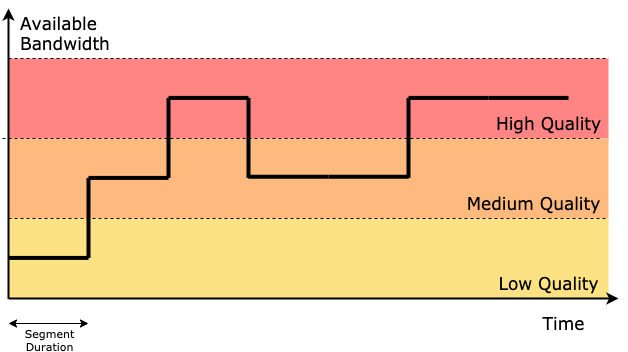
\includegraphics[width=0.7\textwidth]{img/abrtime.png}
  \caption{Evolution of segment quality with time}
  \label{fig:abrtime}

\end{figure}

But there was no official standarization for adaptive video delivery over HTTP. For that reason,
a new international stadard called \textit{MPEG-DASH} was developed and published.

\section{Dynamic Adaptive Streaming over HTTP}
\label{sec:dash}

\textit{DASH} was developed from January 2009 to March 2010 and published in April 2012. 
The most recent revision of the standarization was released in 2019 as 
\textit{MPEG-DASH ISO/IEC 23009-1:2019} \cite{ISO23009}. 
 \textit{Moving Picture Experts Group} from \textit{ISO/IEC} and the \textit{3GPP} collaborated on
the \textit{DASH} standard. The \textit{3\textsuperscript{rd} Generation Partnership Project} defined the use of
\textit{DASH} as the standard of digital media delivery in mobile networks (4G \textit{LTE}, 5G) in \cite{3gpp1}.

The objective of \textit{DASH} was to create a unique standard that replaces the propietary solutions
from Microsoft, Apple and Adobe. Also, it will offer the interoperability and the convergence needed for 
the expansion of large-scale video streaming solutions. Also, the \textit{DASH Industry Forum (DASH-IF)} was created to promote and help the expansion of
\textit{DASH}. Microsoft, Apple, Netflix, Qualcomm, Ericsson and Samsung are some of the companies
members of the \textit{DASH-IF}.

One of the biggest advantages of \textit{DASH} is that the video streaming is over \textit{HTTP} version 1.1 protocol
(\textit{HTTP/1.1}). The use of \textit{HTTP} means that reusing existing internet infrastructure and
media content distribution tecniques using \textit{CDN (Content Delivery Networks)} can be done.
Another convenience of using \textit{DASH} is that due to using \textit{HTTP} encapsulation, problems
with passing through firewalls and the \textit{Network Address Translation (NAT)}
are not existent.

All the control of the media content delivery is located in the \textit{DASH} client side. The
standard does not define any web delivery mechanism nor the bitrate adaptation algorithm. What \textit{DASH}
does define in \cite{ISO23009} are:

\begin{itemize}
  \item \textit{\textbf{The Media Presentation Description (MPD) File Format}}: The \textit{MPD} file
  uses the \textit{eXtensible Markup Language (XML)} and
  contains the specifications of the media content and the \textit{URL} of the segments
  in the \textit{HTTP} video servers.
  \item \textbf{Segment format}: \textit{DASH} defines the characteristics of the necessary
  codifications and the way that the media content is divided in small fragments called 
  \textit{segments}.
\end{itemize}


\begin{figure}[h]
  \centering
  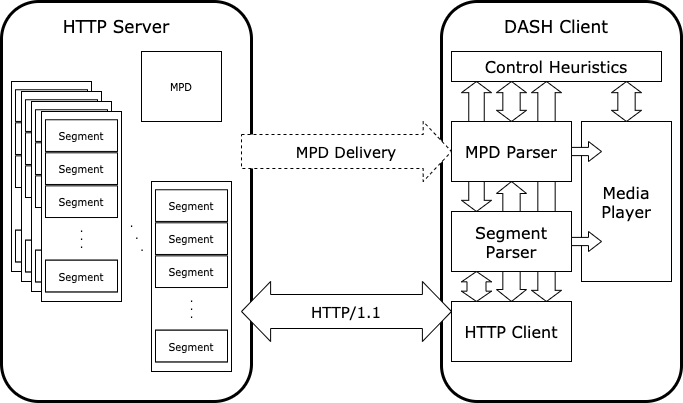
\includegraphics[width=0.7\textwidth]{img/dasharch.png}
  \caption{DASH client-server architecture. Source: MPEG \cite{ios1}}
  \label{fig:dasharch}
\end{figure}

The \autoref{fig:dasharch} presents a simple \textit{DASH} architecture. The video and audio
content are processed and stored on an \textit{HTTP} server. To access the content, the client
sends \textit{HTTP} requests to the server. But first, the client needs to download the 
\textit{MPD} file, normally through \textit{HTTP}. The client then does the
parsing of the \textit{MPD}, extract information such as the duration of a segment, media types or 
resolutions. Finally, the \textit{DASH} client chooses the adequate quality and starts the 
streaming of the content using \textit{HTTP GET} request to fetch the segments.

The \textit{DASH} client stores the segments in a buffer and consumes the content. It continues
to fetch new segments and by monitoring network variables it will decide which quality (higher
or lower bitrate) to request next to avoid problems like buffer underflow and maintain at 
least a set number of segments in the buffer.

\subsection{MPD}
\label{sec:mpd}
The \textit{MPD} file is an \textit{XML} document that describes the characteristics
of the different media components that composes the media content (e.g. video, audio, subtitles).

The structure of the \textit{MPD} is hierarchical as illustrated in \autoref{fig:mpd}. The media content is divided in a sequence of
\textbf{periods}, each period has a starting time and a duration. In a period, the set of encoded
versions of the media content is consistent, that is, the same bitrates, languages and so on.

\begin{figure}[h]
  \centering
  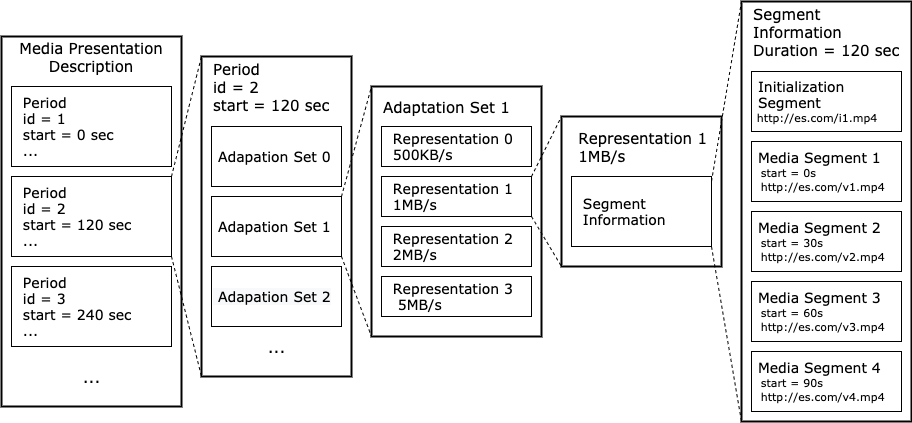
\includegraphics[width=\textwidth]{img/mpd.png}
  \caption{The MPD hierarchical data model. Source: MPEG \cite{ios1}}
  \label{fig:mpd}
\end{figure}

Each period consists of one or multiple \textbf{adaptation sets}. A collection of interchangeable 
encoded versions of one or more media content components is referred to as an adaptation set. For instance,
and adaptation set may contain the different bitrates of the video component of the same multimedia content
and another adaptation set may contain the different bitrates of the audio component of the same multimedia
content.

An adaptation set contains a set of \textbf{representations}. A representation describe an enconded
alternative of the same media component, the alternatives can vary by bitrate, resolution, framerates, 
codec, sampling rate or other characteristics.

Each representation consists of one or multiple \textbf{segments}. A segment is the media stream chunks
in temporal sequence. Each segment has a \textit{URI}, the client will use this \textit{URI} to make
\textit{HTTP GET} requests to the video server. 


\subsection{Adaptation Algorithms}
\label{sec:adap}

In a video streaming service, there are a number of factors like the download bandwidth, delay or packet losses
that can produced undesirable effects on the client such as buffer underflow, rebuffering and interruptions
that lead to bad playback experience, thus, a bad Quality of Experience. To solve these problems, the ABR video
streaming clients uses different adaptation algorithms to give a higher QoE.

An adaptation algorithm is a technique used in a multimedia streaming service to adjust the video quality
in real-time according to different parameters. Some of the parameters are:

\begin{itemize}[noitemsep,topsep=0pt]
  \item \textbf{Client device}: The screen resolution, CPU capabilities, Buffer size, etc.
  \item \textbf{Network}: Type of access network (Mobile, Fixed), available bandwidth, etc.
\end{itemize}

The following subsections will explain different types of adaptation algorithms and the algorithms implemented
for this thesis in \textit{ns-3}.

\subsubsection{Bandwidth throughput based algorithms}

This group of algorithms uses estimations of bandwidth throughput as the main rule to select
the qualities of the multimedia content for the client. The main difference between algorithms of
this kind is the bandwidth estimation method and how the estimation relates to the qualities. 

\begin{figure}[h]
  \centering
  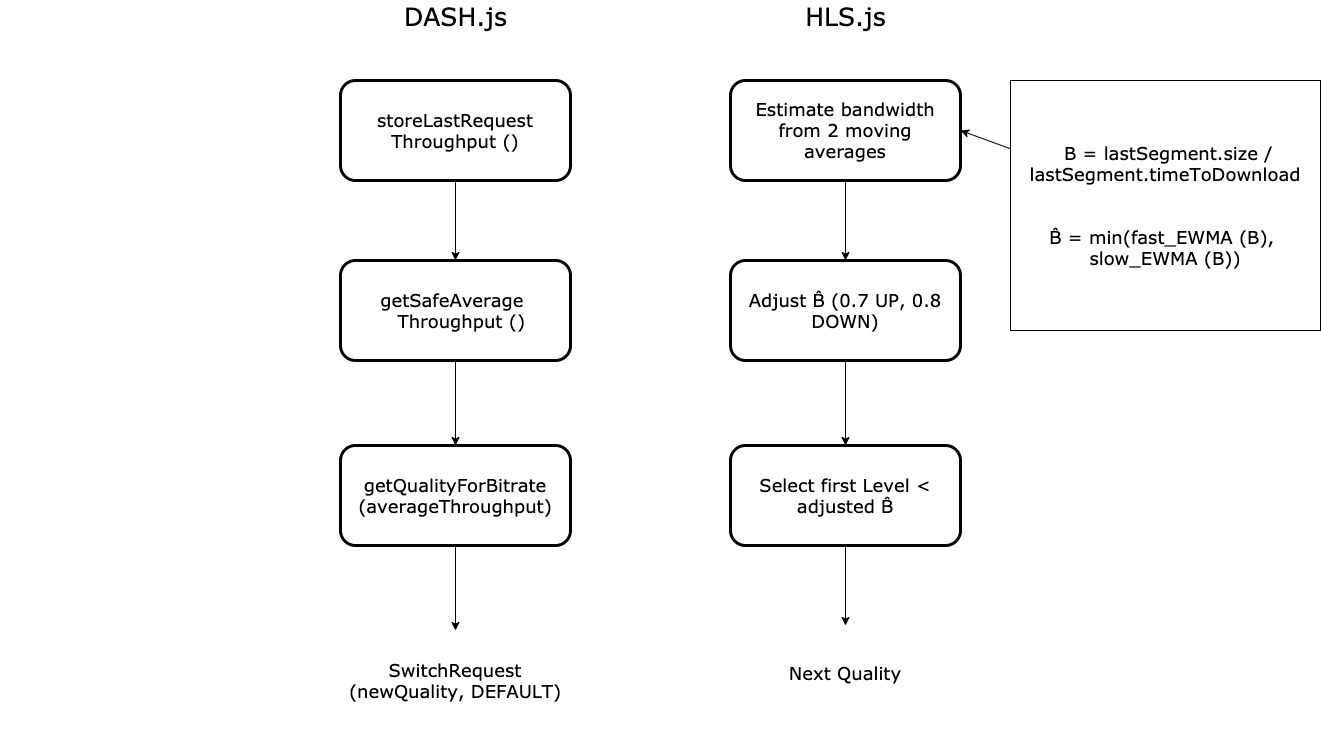
\includegraphics[width=\textwidth]{img/dashjs.png}
  \caption{Bandwidth based algorithms. Source: \cite{abr1}}
  \label{fig:throughput}
\end{figure}

\begin{itemize}
  \item \textbf{HLS.js} \cite{hls3}. The algorithm is called Bandwidth estimation. 
  
  The algorithm processes two EWMA (Exponentially Weighted Moving Averages) and chooses the minimum of the two 
  as the bandwidth estimation.
  Then the bandwidth estimation is multiplied by a factor to reduce oscilation. And finally it selects the 
  first quality with a bitrate less than the adjusted bandwidth estimation. 


  \item \textbf{DASH.js} \cite{dash3}. The Throughput Rule.
  
  This algorithm is basically the same as the Bandwidth estimation from HLS.js.
  It computes the average throughput, and uses an safety factor to avoid oscilations. And then chooses the quality
  based on the safe average and creates a new \textit{SwitchRequest}.

  
\end{itemize}

\subsubsection{Buffer based algorithms}

This group of algorithms uses buffer occupancy information to try to choose the highest level of bitrate
for the multimedia content. These algorithms are usually used to avoid buffer underflow.

\begin{itemize}
  \item \textbf{BOLA} \cite{bola1}. Buffer Occupancy based Lyapunov Algorithm.
  
  The BOLA adaptation algorithm uses the Lyapunov optimization to make decisions. This is an utility 
  theory and it is configurable with a tradeoff parameter to choose between rebuffering potential and bitrate
  maximization.
  
  \begin{figure}[h]
    \centering
    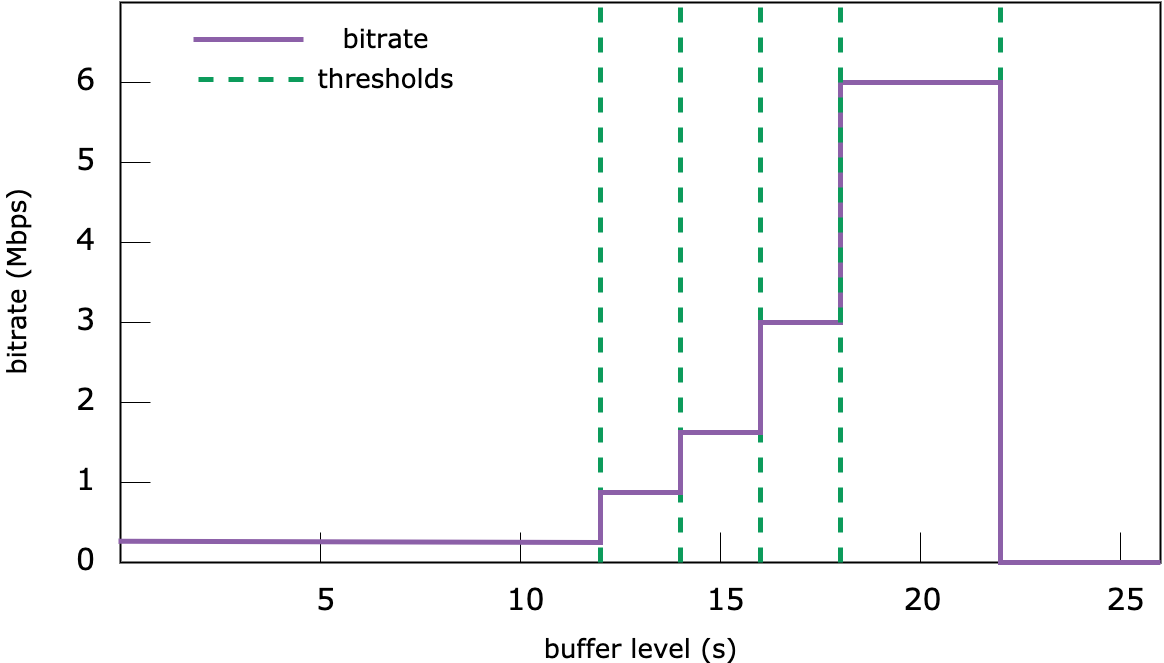
\includegraphics[width=0.75\textwidth]{img/BOLA.png}
    \caption{BOLA's bitrate choice as function of buffer level. Source: \cite{bola1}}
    \label{fig:bola}
  \end{figure}

  BOLA tries to maximize ${V_{n}+\gamma S_{n}}$.
  where: 
  \begin{itemize}
    \item[$\circ$] \textbf{${V_{n}}$} is the bitrate utility.
    \item[$\circ$] \textbf{${S_{n}}$} is the playback smoothness.
    \item[$\circ$] \textbf{${\gamma}$} is the tradeoff weight parameter.
  \end{itemize}
\end{itemize}


\subsubsection{Control theory based or hybrid algorithms}

This class of algorithms uses a combination of throughput estimation and buffer occupancy and tries to 
maximize the bitrate selection with decision-taking indicators calculated making use of control theory or
stochastic optimal control equations.

\subsection{QoS \& QoE Metrics}
\label{sec:qoemetrics}


The \textit{Quality of Service (QoS)} is defined by the \textit{ITU-T} in the document P.10/G.100
 \cite{itu2} as \textquotedbl The totality of characteristics of a telecommunications service that bear on its 
 ability to satisfy stated and implied needs of the user of the service\textquotedbl. And the \textit{Quality of 
Experience (QoE)} is defined as \textquotedbl The degree of delight or annoyance of the user of an application or service\textquotedbl.

The standard \textit{ISO/IEC 23009} defines a list of parameters for \textit{Quality of Service (QoS)} and
\textit{Quality of Experience (QoE)} for the adaptation algorithms to base on. There parameters 
is also used to evaluate the overall quality in the multimedia distribution service.

Some of the metrics defined in \cite{3gpp1} and \cite{ISO23009} are as follows:

\begin{itemize}
  \item \textbf{Average Throughput}: This is a \textit{QoE} metric that defines a list in which 
  the average Throughput observed in the client during a measuring period.
  \item \textbf{Initial Playout Delay}: This is a \textit{QoE} metric that represents the initial 
  delay in the reproduction of the media content.
  \item \textbf{Representation Switch Events}: This is a \textit{QoS} metric for measuring the 
  number of representation switch events of the multimedia content.
  \item \textbf{Buffer Level}: This is a \textit{QoS} metric that monitors the level of occupancy
  of the buffer during the reproduction of the multimedia content.
\end{itemize}


\section{LTE}
\label{sec:4g}

\textit{Long Term Evolution (LTE)} was first introduced in 2008 in the Release 8 of the \textit{3GPP}
specification \cite{lte1}. The objective of \textit{LTE} was to migrate the \textit{3GPP} systems
into a optimized system based on packet switching (all \textit{IP}), with greater bitrates, lower
latency y multiple radio access technologies support.

\subsection{History}
\label{sec:4gintro}

The first mobile phone call was made in 1973 \cite{mob1}. New generations of mobile networks 
are developed almost every decade. The first generation 1G launched years later, but
it was only capable of doing voice calls. In 1991, the second generation 2G \textit{(GSM)} of 
mobile networks was introduced. \textit{GSM} provided improved wireless capabilities and 
introduced by the first time multimedia content with \textit{Multimedia Message Service (MMS)}.
But it was the third generation 3G, launched in 2001, that enabled new internet-driven
services such as video conferencing and streaming. Later in 2009, the \textit{LTE} 4G standard
was commercially deployed. With theorical download bandwidth of almost 100Mbps made high-quality
streaming into reality. 5G technologies improves in bandwidth even more and brings 
video streaming in \textit{UHD} and more.

The consumption of multimedia content on mobile networks is becoming increasingly relevant with 
the rise of bandwidth and ease of access. This section will provide a brief introduction to the 
basic concepts of mobile networks, their architecture and fundamentals.

\subsection{Architecture}
\label{sec:eps}

The design of the \textit{LTE} architecture was done from the ground up. The goal was to build a flat, all
\textit{IP} architecture using packet-switching, well structured (separation of control plane and user plane)
and with few elements.

\begin{figure}[h]
  \centering
  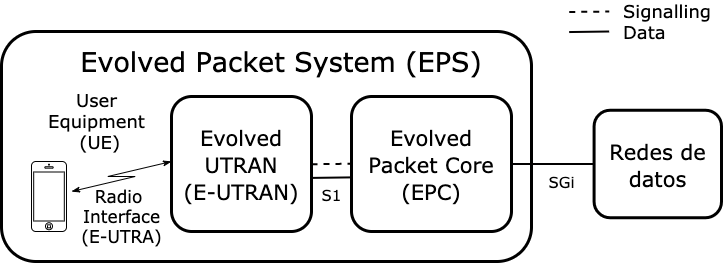
\includegraphics[width=0.8\textwidth]{img/eps.png}
  \caption{LTE Architecture}
  \label{fig:eps}
\end{figure}

The \textit{Evolved Packet System (EPS)} is constituted by the following elements:

\begin{itemize}
  \item \textbf{\textit{User Equipment (UE)}}: An \textit{UE} is any device used by an end user
  to communicate in a mobile network.
  \item \textbf{\textit{Evolved UMTS Terrestial Radio Access Network (E-UTRAN)}}: The only elements
  in the \textit{E-UTRAN} are the \textit{e-NodeB}. An \textit{\textbf{enhanced Node B (e-NodeB)}} works as a base station
  and a controller.
  \item \textbf{\textit{Evolved Packet Core (EPC)}}: The \textit{EPC} is made up of a network of gateways, 
  control servers, and databases linked by a \textit{IP} backbone. The main elements of the \textit{EPC}
  are:
  \begin{itemize}
    \item[$\circ$] \textit{\textbf{Mobility Management Entity (MME)}}: The \textit{MME} is a server 
    used for managing the signalling of the operation. 
    \item[$\circ$] \textit{\textbf{Serving Gateway (SGW)}}: The \textit{SGW} is the gateway used for
    communicating the access network \textit{E-UTRAN} and the \textit{PGW}.
    \item[$\circ$] \textit{\textbf{Packet Data Network Gateway (PGW)}}: The \textit{PGW} is the gateway
    for the traffic between the core network and external packet data networks. 
    \item[$\circ$] \textit{\textbf{Home Subscriber Server (HSS)}}: The \textit{HSS} is a database 
    containing information about the \textit{EPC} network users.  
    \item[$\circ$] \textit{\textbf{Policy Charging and Rule Function (PCRF)}}: The \textit{PCRF} is used
    for \textit{QoS}, policy and charging management. 
  \end{itemize}
\end{itemize}

\begin{figure}[h]
  \centering
  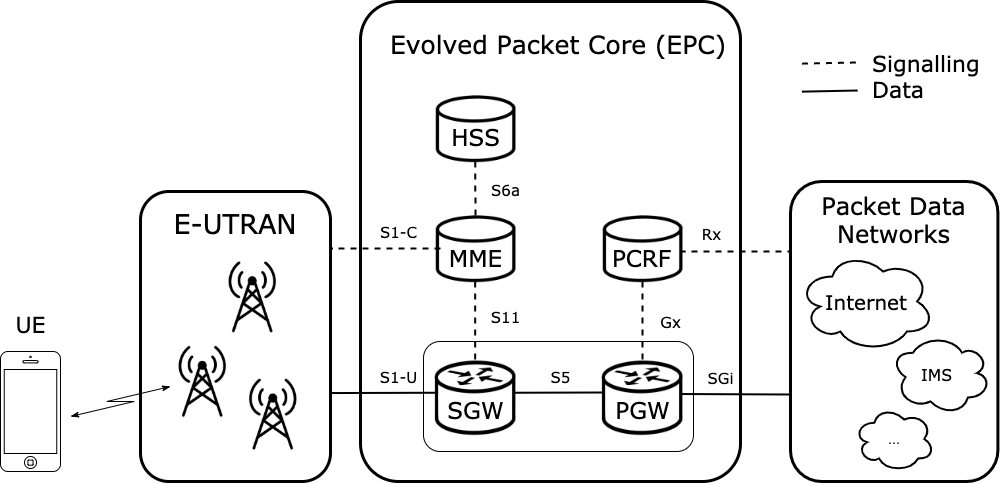
\includegraphics[width=0.8\textwidth]{img/epc.png}
  \caption{Evolved Packet Core (EPC) Architecture}
  \label{fig:epc}
\end{figure}

\subsection{OFDMA and SC-FDMA}
The cellular communication systems needs to have a strategy for multiple access. In LTE, the 
\textit{Orthogonal Frequency Division Multiple Access (OFDMA)} is used for downlink and the \textit{Single-
Carrier Frequency Division Multiple Access (SC-FDMA)} is used for uplink. Both are very similar, consisting
in allocating each subscriber some portion of the subcarriers for certain amount of time.

In the Figure \ref{fig:lterb}, a transmission structure of LTE is presented. The two dimentions of the 
plane are time and frequency. Two important concepts are defined as:

\begin{figure}[h]
  \centering
  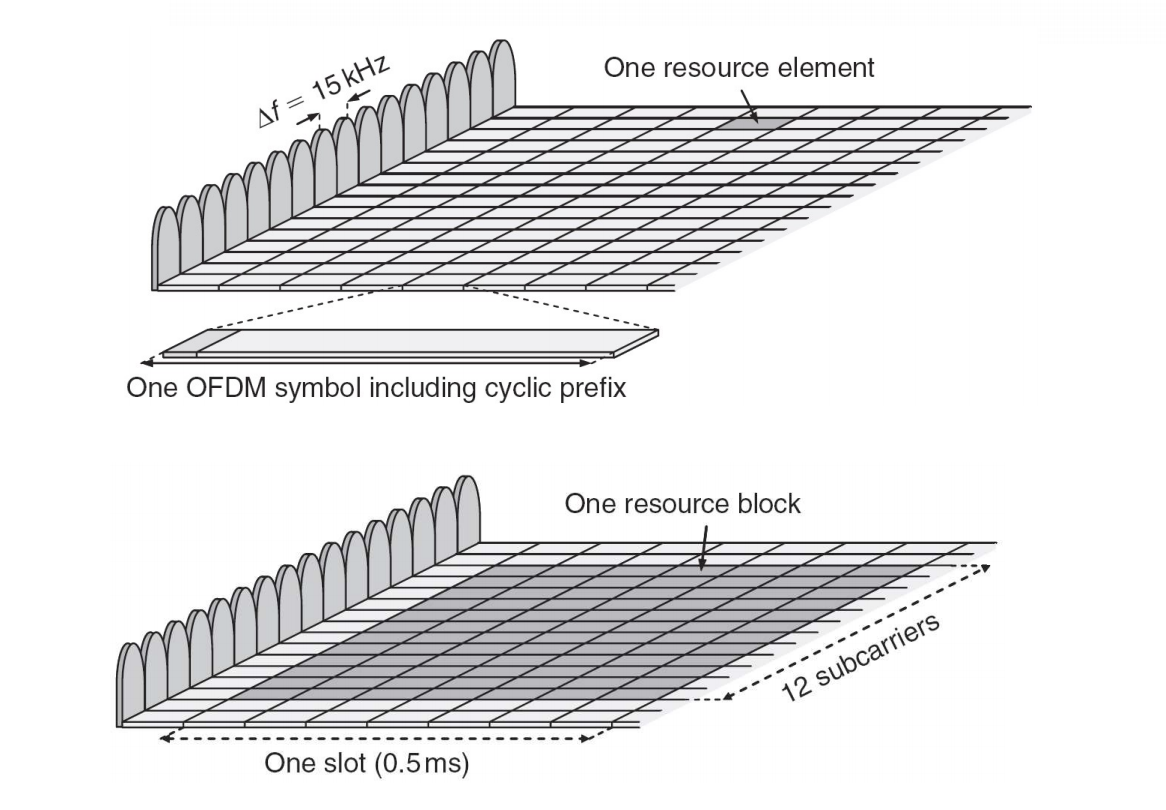
\includegraphics[width=0.95\textwidth]{img/lte_rb.png}
  \caption{LTE Time-Frequency Grid. Source:\cite{cmov1} }
  \label{fig:lterb}
\end{figure}

\begin{itemize}
  \item \textbf{\textit{Resource Element (RE)}}: A Resource Element is the basic element of resouce, it is
  defined as one subcarrier in a symbol period.
  \item \textbf{\textit{Resource Block (RB)}}: A Resource Block is composed by twelve subcarriers (180 kHz) in 
  a time interval of 0.5 ms (7 OFDM symbols).
\end{itemize}


Users are assigned resources in resource blocks across a subframe, i.e., 12 subcarriers over ${2\times7 = 14}$
OFDM symbols for a total of 168 Resource Elements. Because some of the 168 resource components are utilized 
for various layer 1 and layer 2 control messages, not all of them can be used for data.

The number of Resource Blocks available for each channel bandwidth is given by the Table \ref{table:rb}. 

\begin{table}[h]
  \centering
  \begin{tabular}{@{}lcccccc@{}}
  \toprule
  \textbf{Bandwidth}               & 1.4 MHz & 3 MHz & 5 MHz & 10 MHz & 15 MHz & 20 MHz \\ \midrule
  \textbf{Number of RBs available} & 6       & 15    & 25    & 50     & 75     & 100    \\ \bottomrule
  \end{tabular}
  \caption{Number of Resource Blocks against each channel bandwidth. Source: \cite{ofdma1}}
  \label{table:rb}
\end{table}


\subsection{Wireless Fundamentals}

Large-scale wireless networks, such as LTE, are fundamentally inefficient and prone to 
interference. Supporting mobility while also obtaining high levels of power efficiency, 
such as through directional antennas, can be really challenging. Base stations must be 
selectively installed but accommodate vast user populations in order to be cost-effective, 
resulting in a significant amount of self-interference. As a result, achieving high coverage, 
capacity, and dependability at low cost and used power is extremely difficult, if not impossible.

The following list highlights the main parameters affecting the received signal in a wireless system. 


\subsubsection{Propagation loss} 

The amount of transmitted power that actually reaches the receiver is the first visible 
difference between wired and wireless channels. The transmitted signal energy extends along 
a spherical wavefront if an isotropic antenna is utilized, hence the energy received at an 
antenna ${d}$ distant is inversely proportional to the sphere surface area, ${4\pi d^2}$.
However, in reality the propagation environment is not free space, we may also take into
account other factors such as reflections.

\subsubsection{Shadowing} 

Obstacles such as trees and buildings, as shown in Figure \ref{fig:pathloss}, may be situated between the 
transmitter and receiver, causing temporary signal degradation, whereas a temporary line-of-sight 
transmission path would result in abnormally high received power.

\begin{figure}[h]
  \centering
  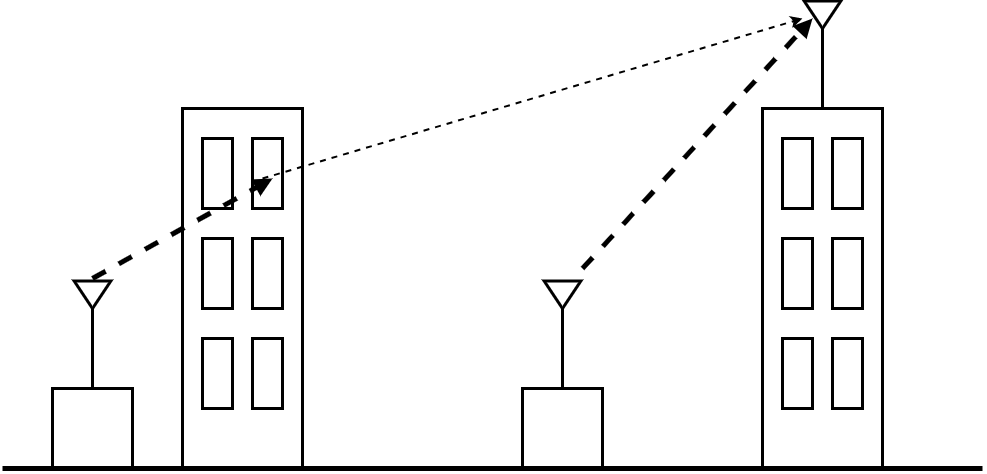
\includegraphics[width=0.77\textwidth]{img/pathloss.png}
  \caption{Shadowing effect. Source:\cite{lte2} }
  \label{fig:pathloss}
\end{figure}

\subsubsection{Fading loss} 

The fading effect is another aspect of wireless channels. Fading is generated by the receiving 
of multiple versions of the same signal (multipath), unlike path loss or shadowing, which are large-scale 
attenuation effects induced by distance or obstacles.

The reflections may arrive at very short intervals. For example, if there is local dispersion 
around the receiver, or they may arrive at relatively longer intervals, for instance, if the 
transmitter and receiver are on multiple pathways. Figure \ref{fig:fading} illustrates this.

\begin{figure}[h]
  \centering
  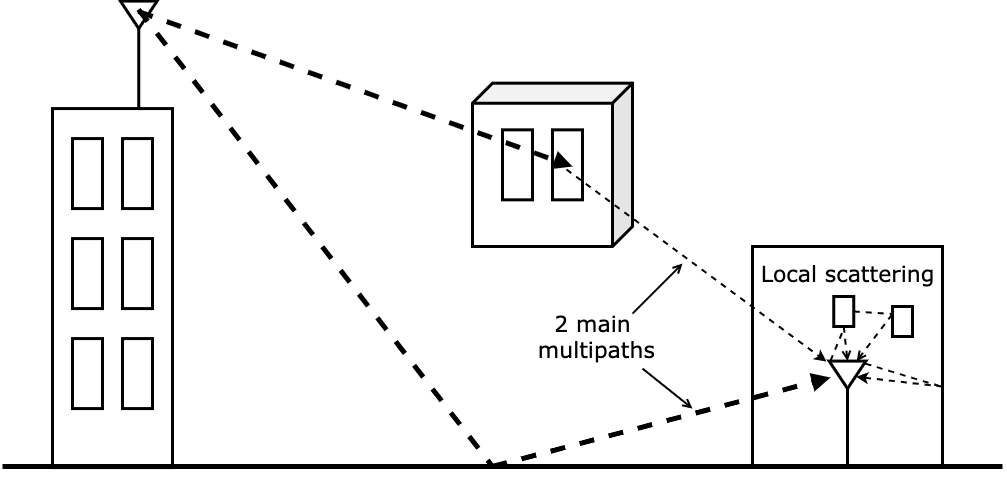
\includegraphics[width=0.77\textwidth]{img/fading.png}
  \caption{Fading loss effect. Source:\cite{lte2} }
  \label{fig:fading}
\end{figure}

\subsection{Antennas \& MIMO}

An antenna is a device that uses electromagnetic waves to transmit or receive information.
The transmitting antenna turns electrical currents into electromagnetic waves, 
and vice versa (receiving antenna).

\textit{Multiple Input, Multiple Output (MIMO)} is a technique for increasing the capacity 
of a radio link by employing multiple transmitting and receiving antennas to take advantage
of multipath propagation. MIMO has become a key component of wireless communication technologies 
such as LTE.

There are also special cases of MIMO:
\begin{itemize}[topsep=0pt]
  \item \textbf{\textit{Multiple-input single-output (MISO)}}: When there are multiple transmitting antennas and a single antenna.
  \item \textbf{\textit{Single-input multiple-output (SIMO)}}: When the transmitter has a single antenna and there are multiple receiving antennas.
  \item \textbf{\textit{Single-input single-output (SISO)}}: SISO is a radio system in which neither the transmitter nor the receiver has multiple antennas.
\end{itemize}

Another special type of MIMO is called \textit{Multi User-Multiple Input Multiple Output}.
Single-user SU-higher MIMO's per-user throughput is better suited to more sophisticated user devices with more antennas, 
whereas MU-MIMO is more practical for low-complexity mobile phones with a small number of reception antennas.

\subsection{Physical Layer}

MAC Scheduler
AMC
CQI

mcs

LTE enb phy

RLC: Transparent Mode (TM), Unacknowledged Mode (UM) and Acknowledged Mode (AM)

EARFCN stands for E-UTRA Absolute Radio Frequency Channel Number

SRS periodicity
\chapter{Network Simulator 3}
\label{sec:ns3}



REM

MIMO

LTE enb phy

UM buffer size

TCP new reno?

Lossmodel

Fading loss model

Earfcn


Building
\chapter{ABR Module for ns-3}
\label{chap:abrmodule}

This chapter will introduce a new module for \textit{ns-3} for ABR streaming simulation.
The \autoref{sec:abrobj} will set the objective and the scope of the design. 
The \autoref{sec:abrarch} will present the architecture of the module.
The \autoref{sec:abrmodels} will go over the models the module is composed of.
Finally, the \autoref{sec:abralgo} will explain the adaptation algorithms implemented in this module.


\section{Design Objectives}
\label{sec:abrobj}
The main objective of this chapter is to design and implement a \textit{ns-3} module able 
to simulate the behavior of video streaming devices in mobile network scenarios. To build 
a framework capable of testing new adaptation algorithms and be possible to extract metrics 
to measure quality of services and quality of experience.

\section{Architecture}
\label{sec:abrarch}

The ABR module provides:
\begin{itemize}[noitemsep,topsep=0pt]
  \item \texttt{\textbf{AbrClient}}. This class mimics a video streaming application. It has an instance 
  of \texttt{AbrAlgorithm}, which is responsible of 
  deciding which quality of media content to download from the \texttt{AbrServer}.
  It is an implementation of \texttt{ns3::Application}.
  \item \texttt{\textbf{AbrServer}}. This class simulates a video streaming HTTP server. It receives
  requests from clients and sends the multimedia segments requested. It is an implementation of 
  \texttt{ns3::Application}.
  \item \texttt{\textbf{AbrVariables}}. This class is used for storing common variables between the clients
  and the servers. It contains the definition of Segment, Representation, AbrTask, etc.
  \item \texttt{\textbf{AbrHelper}}. This is a Helper class for the ABR module. It is the responsible 
  for managing the instances of the ABR clients and servers. In addition, \texttt{AbrHelper} can be
  used for extracting QoS and QoE metrics.
  \item \texttt{\textbf{AbrAlgorithm}}. This is a base class to be implemented with different 
  adaptation algorithms.
  \item \texttt{\textbf{HLSjs}}. This is an implementation of \texttt{AbrAlgorithm} based on \cite{hls3}.
  \item \texttt{\textbf{DASHjs}}. This is an implementation of \texttt{AbrAlgorithm} based on \cite{dash3}. 
  It also contains the implementation of the buffer based BOLA algorithm.
  \item \texttt{\textbf{abr-example.cc}}. An basic example script with two nodes linked with a
  \texttt{PointToPoint} connection and a unstable connection.
\end{itemize}

\begin{figure}[]
  \centering
  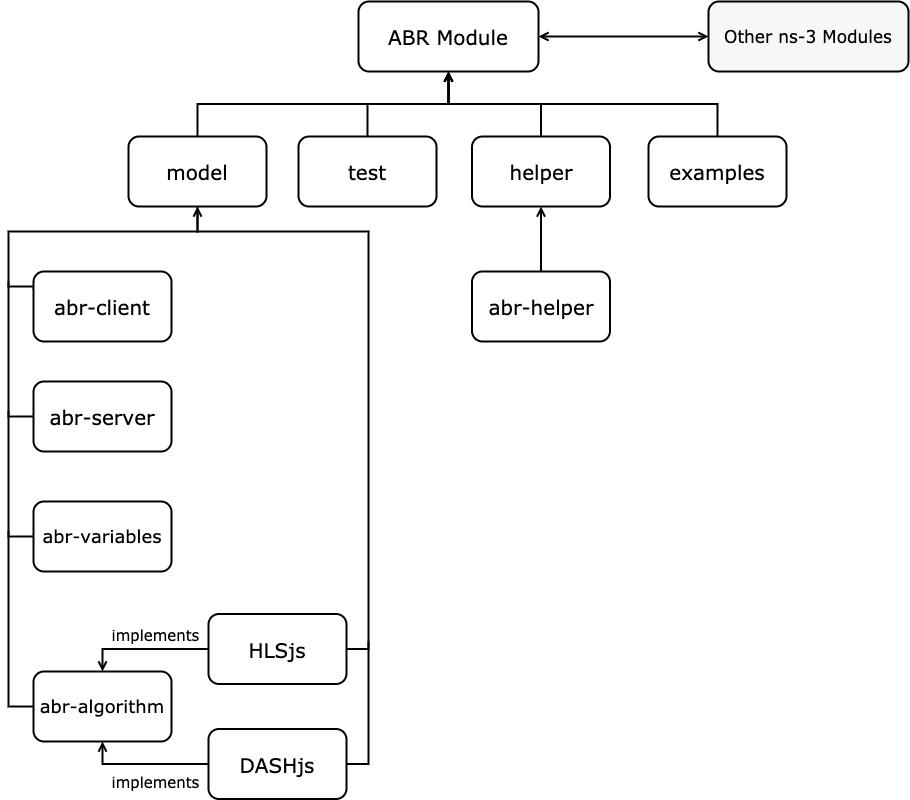
\includegraphics[width=\textwidth]{img/abr.png}
  \caption{ABR Module architecture.}
  \label{fig:abrarch}
\end{figure}

The \autoref{fig:abrarch} shows the architecture of the ABR module. Although this module 
was designed to be used in mobile environments, it can be used with any other \texttt{Application} 
class in \textit{ns-3}, meaning that the ABR clients and servers can be installed in any \texttt{Node}
and work with other \textit{ns-3} modules and models.


\section{Models}
\label{sec:abrmodels}
This section will go through all the models, classes and helpers in the ABR module and how they work 
together.


\subsection{AbrClient}
The \texttt{AbrClient} is an implementation of \texttt{ns3::Application}. This class 
uses an implementation of \texttt{AbrAlgorithm} to create HTTP-like requests to the 
\texttt{AbrServer} and mimics the playing of the media content.

The \texttt{AbrClient} is created with the \texttt{AbrHelper} and the server address and port as
parameters.
Then the client application needs to be installed
on the client nodes. When the simulation starts, the function \texttt{StartApplication} is called
and the simulator is scheduled to call \texttt{HandlePlay} function to simulate video watching.
The client will create a new socket, in this case a TCP socket, to connect with the server.
The socket is set will various callback functions:
\begin{itemize}[noitemsep,topsep=0pt]
  \item \texttt{ConnectionSucceded}. is called if the connection succeeded. Then it calls
  the \texttt{CheckAlgorithm} function.
  \item \texttt{ConnectionFailed}. is called if the connection failed. This should not 
  happen if the simulation script is correctly written.
  \item \texttt{HandleRead}. is called when new packets are received. It stores the segments 
  to the segment buffer, and checks the adaptation algorithms after one entire segment is downloaded.
\end{itemize}

The \texttt{CheckAlgorithm} method asks the \texttt{AbrAlgorithm} and returns
one or more \texttt{AbrTasks}. The client will call the scheduled 
functions depending on the designated task and delay.

\begin{figure}[]
  \centering
  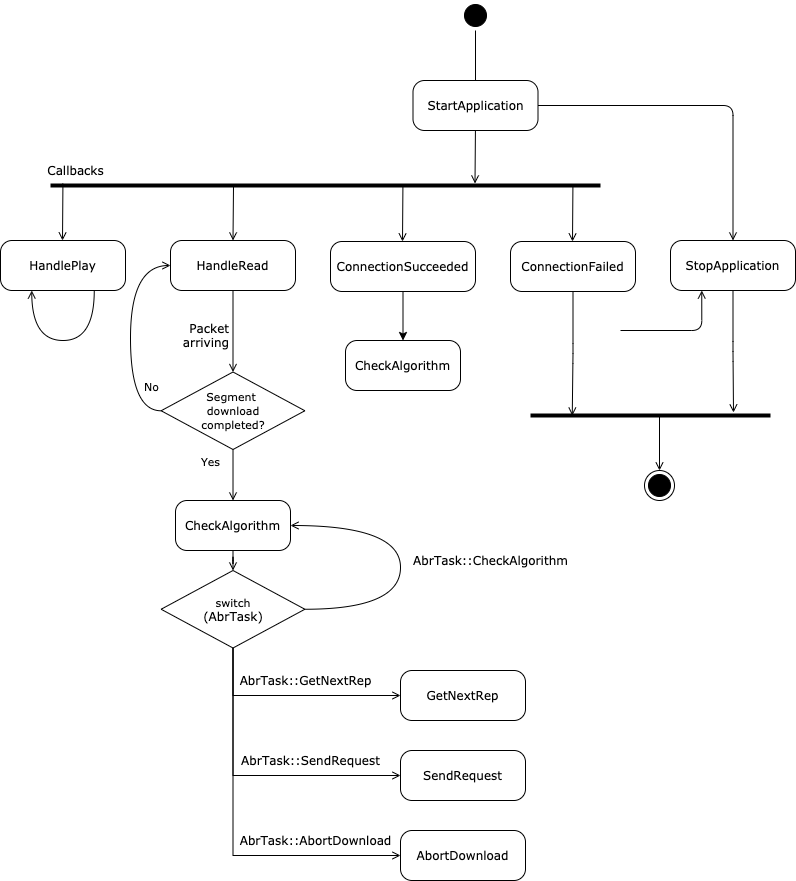
\includegraphics[width=\textwidth]{img/abrclient.png}
  \caption{ABR Client.}
  \label{fig:abrclient}
\end{figure}

\subsection{AbrServer}

The \texttt{AbrServer} is an implementation of \texttt{ns3::Application}. This class 
receives HTTP-like requests from the \texttt{AbrClient} and sends the requested segment.

The request is in the format:

\begin{itemize}[noitemsep, topsep=0pt]
  \centering
  \item[] \texttt{\textbf{GET qualityIndex numberOfSegments startSegment}}
\end{itemize}

For example, "\texttt{GET 4 1 3}" means "GET 1 segment of quality index 4 starting from the 
${3^{rd}}$ segment".


\begin{figure}[h]
  \centering
  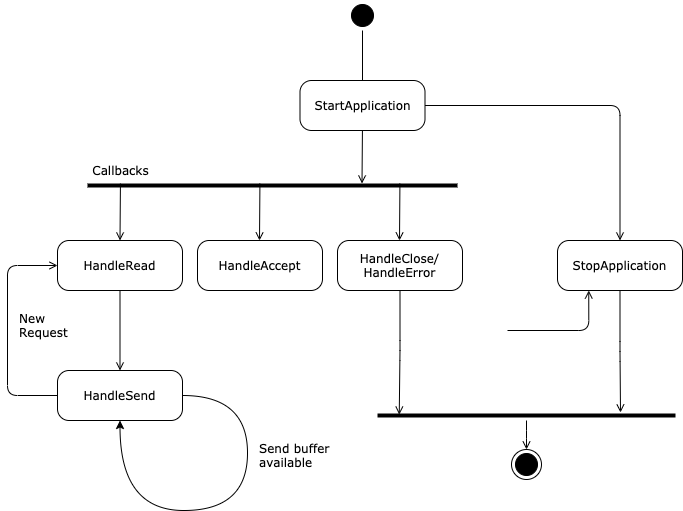
\includegraphics[width=0.95\textwidth]{img/abrserver.png}
  \caption{ABR Server.}
  \label{fig:abrserver}
\end{figure}


The \texttt{AbrServer} is created with the \texttt{AbrHelper} and the listening port as the 
parameter. Then the
server application needs to be installed on the server node. When the simulation starts, the 
function \texttt{StartApplication} is called. The server will create a socket, binds it and starts
to listen.
The socket is set will callback functions. When the sockets are connected, the server 
will schedule new callbacks to handle reading requests and sending data.


\subsection{AbrVariables}

The \texttt{AbrVariables} class contains variables and functions used by the
\texttt{AbrClient} and \texttt{AbrServer}, including the definition of 
a set of essential data structures. These data structures are:

\begin{itemize}[noitemsep, topsep=0pt]
  \item \texttt{\textbf{Segment}}. It is an abstraction of a media segment. A \texttt{Segment} 
  has a size (in bytes), a start time and a duration.
  \item \texttt{\textbf{Representation}}. Describes a certain version of a encoded media. A \texttt{Representation}
  include the resolution, the frames per second and the encoding bitrate.
  \item \texttt{\textbf{SegmentInfo}}. This is a aditional data structure for \texttt{Segment}. A \texttt{SegmentInfo} contains 
  information about download start/finish time, playback start/finish time, the bandwidth estimation
  used to download that segment and the quality index of the segment.
  \item \texttt{\textbf{PlayerStates}}. This class keeps track on the player status.
  \item \texttt{\textbf{AbrTask}}. An \texttt{AbrTask} is a used to schedule tasks for \texttt{AbrClients}.
\end{itemize}

\texttt{AbrVariables} has these variables:
\begin{itemize}[noitemsep, topsep=0pt]
  \item \texttt{\textbf{m\_segments}}. It is a two-dimentional vector containing all the segments 
  for the simulation. Each row has de the same quality and the higher the row index, the higher the
  quality. The segments are ordered in time in the columns.
  \item \texttt{\textbf{m\_representations}}. It is a vector containing all the \texttt{Representations}.
  The row index also means the quality level.
  \item \texttt{\textbf{m\_segmentDuration}}. The duration of the segment in milliseconds. By default, it is ${2000ms}$.
\end{itemize}

Before the simulation starts, the \texttt{AbrVariables} class initializes the
variables. Starting with the representations, there are a predefined set of \texttt{Representations}
by default, but they can be changed in the source file. 
Continuing with the segments, their sizes are calculated based on the resolution,
framerate and the encoding bitrate for each representation. 

Also, the possibility of 
creating a MPD file parser has been considered, but it can be done in the future as an improvement.

\subsection{AbrHelper}

\texttt{AbrHelper} are helper classes providing the functionality of managing the ABR clients and 
servers (creating, setting attribute, etc.). There are two classes, \texttt{AbrServerHelper}
and \texttt{AbrClientHelper}. The \texttt{AbrClientHelper} have methods to extract QoE metrics 
after the simulation ends.

\subsection{AbrAlgorithm}

\texttt{AbrAlgorithm} serves as the base class for the implementations of adaptation algorithms.
In the next section, two implementations of \texttt{AbrAlgorithm} are presented.

\section{Adaptation Algorithms}
\label{sec:abralgo}

This section will present two implementation of \texttt{AbrAlgorithm}. The first one
is based on the JavaScript library implementation of \textit{HTTP Live Streaming (HLS) hls.js}\footnote{\textit{hls.js} will refer to the original JavaScript Library while
\texttt{HLSjs.cc} will refer to the \textit{ns-3} implementation} client \cite{hls3}.
The second implementation is based on the \textit{dash.js} 
\footnote{\textit{dash.js} will refer to the original DASH implementation while
\texttt{DASHjs.cc} will refer to the \textit{ns-3} implementation}
from the \textit{DASH Industry Forum} \cite{dash3}.

\subsection{HLSjs.cc}
This class is based on the implementation from a open-source JavaScript-based project called
\textit{hls.js}.
The \texttt{HLSjs.cc} class has some simplifications compared to the original
library.

\textit{hls.js} has two main rules and some aditional secondary rules. These rules are:
\begin{itemize}[noitemsep, topsep=0pt]
  \item Main Rules
  \begin{itemize}[noitemsep, topsep=0pt]
    \item[$\circ$] \textbf{Bandwidth Estimation}. This is the main rule, which is an ABR adaptation
    algorithm rule explained in the \autoref{sec:adap}.
    \item[$\circ$] \textbf{Abort Rules}. These are a set of rules to abort a segment download depending on
    some coditions, for example, a timeout for a segment to download.
  \end{itemize}
  \item Secondary Rules
  \begin{itemize}[noitemsep, topsep=0pt]
    \item[$\circ$] \textbf{Screen \& player size cap level}. This rule is used at the beginning to cap the highest
    level of representation to the device capabilities. For instance, there is no need for a FHD
    device to play 4K videos in most cases.
    \item[$\circ$] \textbf{Dropped frames per second}. This rule is triggered if the cpu cannot handle the 
    decoding of the multimedia content and produces too much dropped frames.
  \end{itemize}
\end{itemize}

\texttt{HLSjs.cc} will focus only on the Bandwidth Estimation rule. In addition, there is another 
rule called \texttt{BufferRule} that will be explained after.
\lstset{escapeinside={(*@}{@*)}}

\begin{itemize}
  \item \textbf{\texttt{BandwidthRule}}. This is the implementation of a EWMA based adaptation
  algorithm. The \autoref{lst:hls} show a pseudocode of the algorithm.
  \item \textbf{\texttt{BufferRule}}. This rule introduces a delay to the client
  next request based on the buffer status.
\end{itemize}

\subsection{DASHjs.cc}
This class is based on the implementation build by the \textit{DASH Industry Forums} with the \textit{dash.js}
name. \texttt{DASHjs.cc} is a simplified version of \textit{dash.js}. See \autoref{sec:dashjs} for more details.

\textit{dash.js} works with a combination of rules. Each rule returns a \texttt{SwitchRequest}.
A \texttt{SwitchRequest} is an object that indicates, between others, the next representation, the 
request priority, etc. The priorities of the \texttt{SwitchRequest} can be \texttt{NO\_CHANGE}, 
\texttt{DEFAULT}, \texttt{STRONG} or \texttt{WEAK}.

If more than one \texttt{SwitchRequest} is created, the \texttt{GetMinSwitchRequest} is called.
It always considers the request with the highest priority and the quality with the minimum difference compared to the
current representation.

\texttt{DASHjs.cc} has two rules implemented:

\begin{itemize}
  \item \textbf{\texttt{ThroughputRule}}. This is the implementation of a EWMA based adaptation
  algorithm. Is is very similar the the \textit{hls.js} Bandwidth estimation rule.
  

\begin{minipage}{\linewidth}

  \begin{lstlisting}[language=myalgo, caption={HLSjs.cc Bandwidth Rule}, label={lst:hls},captionpos=b]
    if (*@\textit{First Segment}@*) then
      (*@\textit{nextQuality $\leftarrow{}$}@*)0;
      return true;
    end if
    if (*@\textit{Enough segments in buffer}@*) then
      (*@\textit{newSample $\leftarrow{}$}@*) estimation of last segment;
      if (*@\textit{fastEWMA is 0 or slowEWMA is 0}@*) then
        (*@\textit{fastEWMA $\leftarrow{}$ newSample}@*);
        (*@\textit{slowEWMA $\leftarrow{}$ newSample}@*);
      else 
        (*@\textit{fastEWMA $\leftarrow{}$ newSample $\times \,\, \alpha_{fast} + $ fastEWMA $\times \,\, (1 - \alpha_{fast})$}@*);
        (*@\textit{slowEWMA $\leftarrow{}$ newSample $\times \,\, \alpha_{slow} + $ slowEWMA $\times \,\, (1 - \alpha_{slow})$}@*);
      end if
      (*@\textit{averageBw $\leftarrow{}$$ \,\, min($slowEWMA, fastEWMA$ )$}@*);
    else
      (*@\textit{averageBw $\leftarrow{}$}@*) current estimation;
    end if
    for (*@\textit{i = representations.size - 1 \textit{$\rightarrow{}$} 0}@*) do
      if (*@\textit{i < current quality}@*) then
        (*@\textit{adjustedBw $\leftarrow{}$ bwFactor $\times$ averageBw}@*);
      else 
        (*@\textit{adjustedBw $\leftarrow{}$ bwUpFactor $\times$ averageBw}@*);
      end if
      if (*@\textit{adjustedBw > representations[i].bitrate}@*) then
        (*@\textit{nextQuality $\leftarrow{}$i}@*);
        return true;
      end if
    end for
    return false;
  \end{lstlisting}
  \end{minipage}
  
  \item \textbf{\texttt{BolaRule}}. This is the implementation of the buffer based algorithm
  BOLA introduced in \autoref{sec:abralgo}.

  BOLA has three states:
  \begin{itemize}[noitemsep, topsep=0pt]
    \item[$\circ$] \texttt{BOLA\_STATE\_ONE\_BITRATE}. This is the state when there is only one bitrate available.
    \item[$\circ$] \texttt{BOLA\_STATE\_STARTUP}. This is the initial state of BOLA.
    \item[$\circ$] \texttt{BOLA\_STATE\_STEADY}. This is the state when the buffer is really for using BOLA.
  \end{itemize}

  The main methods of BOLA is \texttt{BolaRule} and \texttt{GetQualityFromBufferLevel}.
  This last method uses a score calculated, using BOLA's parameters such as playback utility or 
  playback smoothness, for each representation and chooses the representation
  with the highest score.
\end{itemize}






\chapter{Simulations Scenarios and Results}
\label{sec:scenarios}
% \chapter{Results}
\label{chap:results}
\chapter{Conclusions and Future Work}
\label{chap:conclusions}

\section{Conclusions}

This Master Thesis have the objectives of building a simulation framework
able to test \textit{ABR} adaptation algorithms in mobile network scenarios,
and comparing different implmentations of existing adaptation algorithms 
based on QoE and fairness metrics.

First, the study begin by familiarizing with the simulation software \textit{ns-3}.
It was really challenging at first, due to the lack of grafical user interface
and relatively small community to help solving problems. Learnt scripting
and implementing new modules in \textit{ns-3}.

Also, become familiar the \textit{LTE} technologies. Including the architecture 
of the \textit{EPC}, radio interface, wireless fundamentals and protocol stack layers.
The \textit{LTE} module in \textit{ns-3} made possible the simulation of \textit{ns-3}
applications in mobile scenarios.

To achieve the objectives proposed, the design of a new \textit{ns-3} module is developed.
And also the implementation and integration with other \textit{ns-3} modules. The implemented 
\textit{ABR} module mimics real-world video players behaviour and
can work as a framework to test new adaptation algorithms, and extract
metrics of the simulation. The most difficult part was the implementation of the 
\textit{BOLA} algorithm, it was really complex and hard to understand. An additional
feature was discarted, but can be done in futere work is to parse MPD files as a
input for the simulation.

Finally, various simulations are made to compare \textit{QoE} and fairness metric between
the implemented \textit{ABR} adaptation algorithms. This new module has its limitations
and can be improved with future work. 



\section{Future Work}

These are possible improvements for future work:

\begin{itemize}
  \item \textbf{Implement more adaptation algorithms}. To be able to compared more existing
  adaptation algorithms or even put to test new designs of algorithms.
  \item \textbf{Traffic shapping}. To analyse the effect of applying traffic shapping techniques 
  like token bucket and leaky bucket.
  \item \textbf{TCP congestion control}. As commented on the thesis, the \textit{TCP} congestion 
  control influents the adaptation algorithms. It could be interesting testing scenarios.
  \item \textbf{X2 Handover}. The scripts implemented is limited to one \textit{eNodeB}. There 
  is a possibility in \textit{ns-3} to use multiple \textit{eNodeB} and handover over the \textit{X2}
  interface.
  \item \textbf{5G}. There is a new \textit{5G} module in \textit{ns-3} although in its very 
  early stages. \textit{5G} simulation scenarios could be also worth to look at.
\end{itemize}


\cleardoublepage
\pagenumbering{roman}
\cleardoublepage
\phantomsection
\nocite{*}
\addcontentsline{toc}{chapter}{References}   % ieeetr
% \bibliographystyle{unsrt}
\bibliographystyle{plain}{
    \small
    \bibliography{biblio/ref}
}

\appendix
\renewcommand\chaptername{Appendix}
\begin{appendices}
    \chapter{Impact} \label{chap:impact}


% \section{Socio-economic \& Ambiental Impact} \label{sec:social_impact}

Video traffic continues to grow rapidly, both in terms of overall volume 
and as a percentage of total traffic, especially during this COVID-19
global pandemic. 
Improvements in technology, such as 
4K, 8K video, videoconferences or video-game streaming, and the ever-present 
availability of consumable media, are all contributing to this growth.

The storage and bandwidth costs of transmitting video to these 
increases as streaming services scale up to fulfill the demand for more 
content across more devices. The cost of storing and streaming video may 
be dramatically reduced by 
efficiently providing high-quality video at scale to a wide range of devices, 
while also enhancing playback quality for consumers.

In future years, 5G's speed, capacity, and connectivity will open up a slew of 
possibilities for environmental protection and preservation. Energy efficiency, 
greenhouse gas emissions, and the utilization of renewable energy will all benefit from 
5G technology. Even though 5G technologies are more efficient 
compared to 4G, it is estimated that mobile data will almost fourfold\cite{gsm1} and 
it can be very challenging to reduce the environmental impact the mobile networks
can produce.
    \chapter{Budget} 
\label{chap:economic}

    % \chapter{Example MPD} \label{chap:examplempd}

\lstset{language=XML}

\begin{lstlisting}
<!--  MPD file Generated with GPAC version 0.5.1-DEV-rev5379  on 2014-09-10T13:14:57Z -->
<MPD xmlns="urn:mpeg:dash:schema:mpd:2011" minBufferTime="PT1.500000S" type="static" mediaPresentationDuration="PT0H9M55.46S" profiles="urn:mpeg:dash:profile:isoff-live:2011">
  <ProgramInformation moreInformationURL="http://gpac.sourceforge.net">
  <Title>dashed/BigBuckBunny_1s_simple_2014_05_09.mpd generated by GPAC</Title>
  </ProgramInformation>
  <Period duration="PT0H9M55.46S">
    <AdaptationSet segmentAlignment="true" group="1" maxWidth="480" maxHeight="360" maxFrameRate="24" par="4:3">
      <SegmentTemplate timescale="96" media="bunny_$Bandwidth$bps/BigBuckBunny_1s$Number$.m4s" startNumber="1" duration="96" initialization="bunny_$Bandwidth$bps/BigBuckBunny_1s_init.mp4"/>
      <Representation id="320x240 47.0kbps" mimeType="video/mp4" codecs="avc1.42c00d" width="320" height="240" frameRate="24" sar="1:1" startWithSAP="1" bandwidth="46980"/>
      <Representation id="320x240 92.0kbps" mimeType="video/mp4" codecs="avc1.42c00d" width="320" height="240" frameRate="24" sar="1:1" startWithSAP="1" bandwidth="91917"/>
      <Representation id="320x240 135.0kbps" mimeType="video/mp4" codecs="avc1.42c00d" width="320" height="240" frameRate="24" sar="1:1" startWithSAP="1" bandwidth="135410"/>
      <Representation id="480x360 182.0kbps" mimeType="video/mp4" codecs="avc1.42c015" width="480" height="360" frameRate="24" sar="1:1" startWithSAP="1" bandwidth="182366"/>
      <Representation id="480x360 226.0kbps" mimeType="video/mp4" codecs="avc1.42c015" width="480" height="360" frameRate="24" sar="1:1" startWithSAP="1" bandwidth="226106"/>
      <Representation id="480x360 270.0kbps" mimeType="video/mp4" codecs="avc1.42c015" width="480" height="360" frameRate="24" sar="1:1" startWithSAP="1" bandwidth="270316"/>
      <Representation id="480x360 353.0kbps" mimeType="video/mp4" codecs="avc1.42c015" width="480" height="360" frameRate="24" sar="1:1" startWithSAP="1" bandwidth="352546"/>
      <Representation id="480x360 425.0kbps" mimeType="video/mp4" codecs="avc1.42c015" width="480" height="360" frameRate="24" sar="1:1" startWithSAP="1" bandwidth="424520"/>
      <Representation id="854x480 538.0kbps" mimeType="video/mp4" codecs="avc1.42c01e" width="854" height="480" frameRate="24" sar="1:1" startWithSAP="1" bandwidth="537825"/>
      <Representation id="854x480 621.0kbps" mimeType="video/mp4" codecs="avc1.42c01e" width="854" height="480" frameRate="24" sar="1:1" startWithSAP="1" bandwidth="620705"/>
      <Representation id="1280x720 808.0kbps" mimeType="video/mp4" codecs="avc1.42c01f" width="1280" height="720" frameRate="24" sar="1:1" startWithSAP="1" bandwidth="808057"/>
      <Representation id="1280x720 1.1Mbps" mimeType="video/mp4" codecs="avc1.42c01f" width="1280" height="720" frameRate="24" sar="1:1" startWithSAP="1" bandwidth="1071529"/>
      <Representation id="1280x720 1.3Mbps" mimeType="video/mp4" codecs="avc1.42c01f" width="1280" height="720" frameRate="24" sar="1:1" startWithSAP="1" bandwidth="1312787"/>
      <Representation id="1280x720 1.7Mbps" mimeType="video/mp4" codecs="avc1.42c01f" width="1280" height="720" frameRate="24" sar="1:1" startWithSAP="1" bandwidth="1662809"/>
      <Representation id="1920x1080 2.2Mbps" mimeType="video/mp4" codecs="avc1.42c032" width="1920" height="1080" frameRate="24" sar="1:1" startWithSAP="1" bandwidth="2234145"/>
      <Representation id="1920x1080 2.6Mbps" mimeType="video/mp4" codecs="avc1.42c032" width="1920" height="1080" frameRate="24" sar="1:1" startWithSAP="1" bandwidth="2617284"/>
      <Representation id="1920x1080 3.3Mbps" mimeType="video/mp4" codecs="avc1.42c032" width="1920" height="1080" frameRate="24" sar="1:1" startWithSAP="1" bandwidth="3305118"/>
      <Representation id="1920x1080 3.8Mbps" mimeType="video/mp4" codecs="avc1.42c032" width="1920" height="1080" frameRate="24" sar="1:1" startWithSAP="1" bandwidth="3841983"/>
      <Representation id="1920x1080 4.2Mbps" mimeType="video/mp4" codecs="avc1.42c032" width="1920" height="1080" frameRate="24" sar="1:1" startWithSAP="1" bandwidth="4242923"/>
      <Representation id="1920x1080 4.7Mbps" mimeType="video/mp4" codecs="avc1.42c032" width="1920" height="1080" frameRate="24" sar="1:1" startWithSAP="1" bandwidth="4726737"/>
    </AdaptationSet>
  </Period>
</MPD>
\end{lstlisting}



\end{appendices}

\end{document}